\pdfminorversion=7
\documentclass[12pt, a4paper]{article}

\usepackage[T2A]{fontenc}
\usepackage[utf8]{inputenc}
\usepackage[russian, english]{babel}
\usepackage{multicol}
\usepackage{graphicx}

\title{Reference-Anchored Latent Space Projection for Isolating Disease Signals in Single-Cell Data}
\author{Vladimir Opait \\
\small \textit{Universitat de Valencia}}
\date{}
\begin{document}

\maketitle

\begin{abstract}
Integrating new single-cell cohorts into existing reference atlases is frequently confounded by technical batch effects, which can either obscure or mimic novel biological signals. To address this, we present scGRIP, a Conditional Variational Autoencoder (CVAE) framework designed to decouple batch variations from true disease signatures through reference-guided latent space adaptation. Our approach preserves the geometric and statistical properties of a well-characterized reference latent space using an Anchor Loss alongside standard ELBO optimization. To resolve new cohorts, we apply a Maximum Mean Discrepancy (MMD) objective exclusively to healthy control cells, forcing the alignment of the new healthy population with the reference healthy centroid. This targeted regularization restricts the model's degrees of freedom, compelling it to regress out the technical batch effect rather than biological variance. As a direct mathematical consequence, unaligned populations—cells that remain distant from the healthy centroid in the adapted latent space—naturally emerge as carriers of the disease signal. This geometry-preserving method enables the precise isolation of novel disease states and the robust identification of previously unknown biomarkers in newly integrated data.
\end{abstract}

\begin{figure}[htbp]
    \centering
    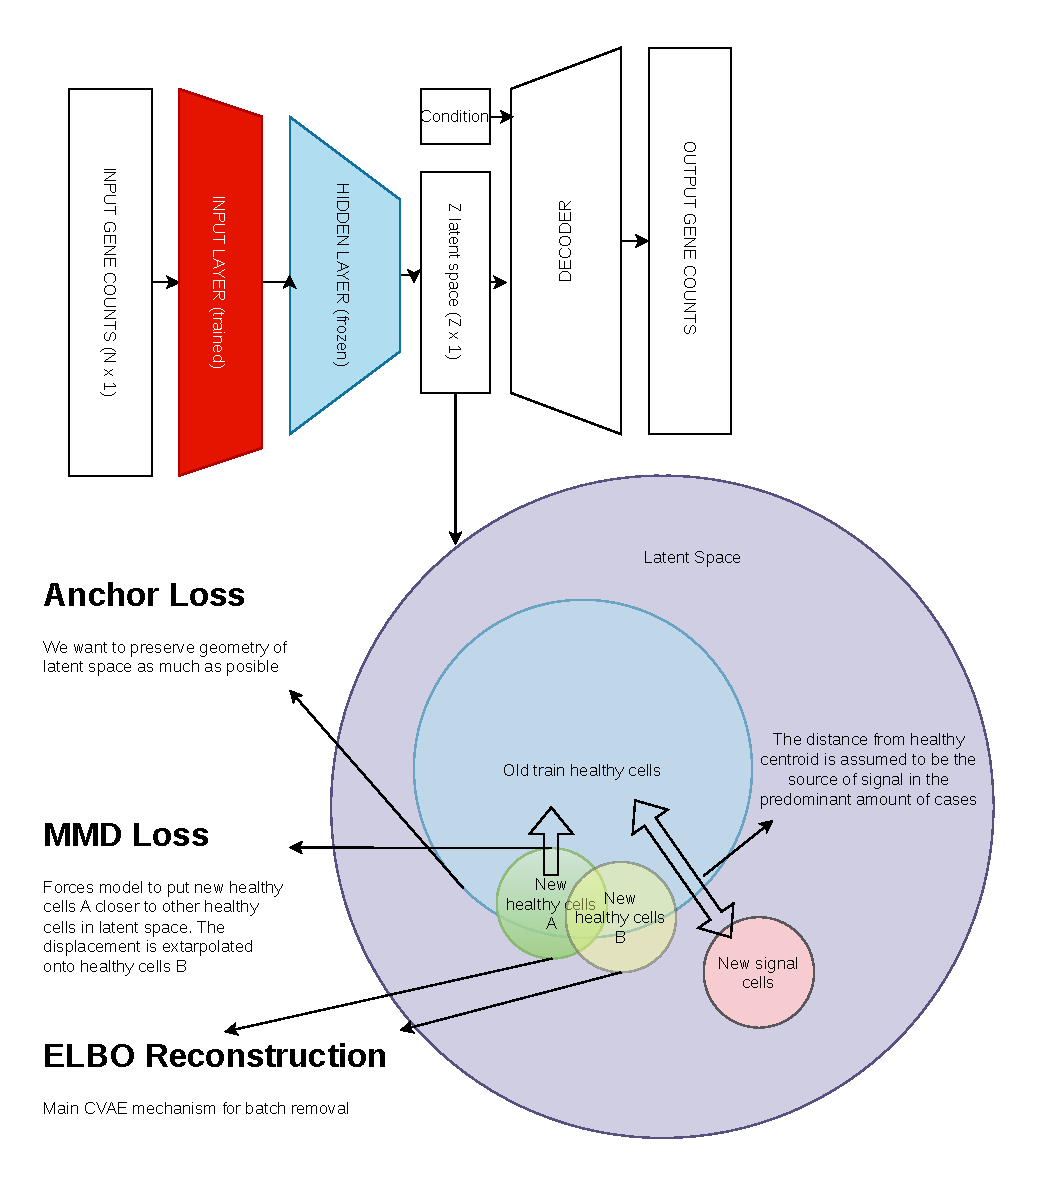
\includegraphics[width=0.8\textwidth]{images/scGRIP_phase1.pdf}
    \caption{Архитектура метода с использованием LoRA и регуляризацией латентного пространства (MMD и Anchor Loss).}
    \label{fig:my_scheme}
\end{figure}

\end{document}